%%% 05-06-2015 updated from 30-04-2015 updated from 02-15-2015
%%% ONLY node and set of nodes robustness measure 
\documentclass[graybox]{svmult}
\usepackage[hang]{footmisc}
%\pagenumbering{arabic}
\setlength{\footnotemargin}{0pt}
\usepackage{footmisc,multicol, graphicx,makeidx,courier,helvet}
\usepackage[latin1]{inputenc}
\usepackage{amssymb,amsmath} 
%\usepackage{mathptmx}
\usepackage{amsfonts}
\usepackage{graphicx}
% choose options for [] as required from the list
% in the Reference Guide

\usepackage{mathptmx}         % selects Times Roman as basic font
\usepackage{helvet}         % selects Helvetica as sans-serif font
\usepackage{courier}        % selects Courier as typewriter font
\usepackage{type1cm}        % activate if the above 3 fonts are
                            % not available on your system
%
\usepackage{makeidx}         % allows index generation
\usepackage{graphicx}        % standard LaTeX graphics tool
                             % when including figure files
\usepackage{multicol}        % used for the two-column index
%\usepackage[bottom]{footmisc}% places footnotes at page bottom
% see the list of further useful packages
% in the Reference Guide

\makeindex             % used for the subject index
                       % please use the style svind.ist with
                       % your makeindex program
\begin{document}
\def\s{\sigma}

%\title*{An informational approach to the Network Disease Hypothesis in resting state fMRI}
\title*{Network efficiency as a classifier for aging in resting
state fMRI}
\author{Jaime Gomez-Ramirez, Yujie Li, Qiong Wu, Xiaoyu Tang, Jinglong Wu}
\institute{Biomedical Engineering Laboratory, Okayama University,  Japan}
%{   Biomedical Engineering Laboratory, Okayama University,  Japan
%\\ Autonomous Systems Laboratory, Universidad Polit�cnica de Madrid, %Spain \\
%{jd.gomez@upm.es}}
 
\maketitle

\abstract{Here we study how network
robustness -functional network invariance under perturbation- is affected upon
the removal of nodes in the functional connectivity network in resting state
(R-fMRI) for both young and elder subjects. We apply analytic measures of network communication efficiency and robustness to R-fMRI in the human brain and explore the capacity of these measures to predict age. 
A new theoretical framework to investigate network robustness and how it is affected by internally driven processes such as aging is provided.
%i.Conclusiones
}
\keywords{resting state fMRI, network degeneration hypothesis, Markov chain,
relative entropy}

\section{Introduction}
The objective of this work is to study network robustness i.e., resilience to
perturbations, in resting state functional connectivity networks.
%Relevance of RS 
It has been suggested that fluctuations in the BOLD signal measured
in humans in resting state, represent the neuronal activity baseline and shape
spatially consistent patterns \cite{Raichle:2005}, \cite{Fransson:2006}. The 
slow fluctuations in the BOLD signal found in resting subjects, are highly
coherent within either structural or functional networks in the human brain.
%Therefore,
%exploring these fluctuations could lead to a better understanding of the
%brain's intrinsic or spontaneous neural activity. %i.But I dont help in this direction in this paper, delete this sentence?
Functional correlation based on the synchrony of low-frequency blood flow
fluctuations in resting state have been identified in the sensorimotor
\cite{kokkonen_preoperative_2009}, visual \cite{damoiseaux_consistent_2006},
language \cite{hampson_detection_2002}, auditory
\cite{hunter_neural_2006}, dorsal and ventral attention
\cite{fox_spontaneous_2006} and the frontoparietal control system
\cite{vincent_evidence_2008}.

%Seed based versus ICA 
The visual identification of the
overall connectivity patters in resting state functional magnetic resonance
imaging (R-fMRI), has been assessed using either model-based and model-free
approaches. In the former, statistical parametric maps of brain activation are
built upon voxel-wise analysis location \cite{biswal_functional_1995}.
While this approach has been successful in
the identification of motor networks \cite{robinson_resting_2009}, it shows important limitations when
the seed voxel cannot be easily identified \cite{maldjian_functional_2001}.
For example, in brain areas with unclear boundaries i.e., cognitive networks
involved for instance, in memory or self processing operations
\cite{fingelkurts_persistent_2011}. 

Independent Component Analysis (ICA), on
the other hand, is a model-free approach that allows separating resting
fluctuations from other signal variations, resulting on a collection of spatial
maps, one for each independent component, that represent functionally relevant networks in the brain
\cite{calhoun_review_2009}.
%Bad sentence, improve style
While ICA has the advantage over model-free methods that it does not need to
assume a specific temporal model of correlation between regions of
interest, the functional relevance of the different components is, however,
computed relative to their resemblance to a number of networks based on
criteria that are not easily formalized \cite{biswal_toward_2010}.

%Graph-based 3ra via 
A third approach, complementary to the other two, which is becoming of paramount importance is the network-based approach. Graph-based techniques have proliferated in the last years providing new
insights into the structure function relationship in the healthy brain, aging and neuropathological disorders \cite{fair_functional_2009}, 
\cite{wang_graph-based_2010}, \cite{he_graph_2010}. 
The use of graph theoretic techniques to model brain networks has shifted the 
emphasis from the identification of local subnetworks -default mode network,
primary sensory motor network etc.- to the quantitative study of the topological
and informational characteristics of large-scale brain networks.
Prove of the utility of this
approach is that notable proponents of a modularist vision of brain
connectivity to understand cognition, such as Gazzaniga
\cite{gazzaniga_new_1999} (see \cite{Fuster:2000} for an early critic of the
modularist approach by Fuster who anticipates a shift toward networks) has
now embraced a complex brain networks approach \cite{bassett_understanding_2011}.

% to understand the interplay
%between structure and function in brain systems 
Network-based approaches to R-fMRI data have demonstrated
non-trivial topological properties of functional networks in the human brain.
Large-scale anatomical
connectivity analysis in the mammalian brain, shows that brain topology is
neither random nor regular. Instead, small world
architectures \cite{Watts:1998} -highly clustered nodes connected thorough
relatively short paths- have been identified in brain networks. 
%\cite{Vaessen:2010}.
Small world networks are not solely
structural, functional networks with a small world organization have been
identified in the mammal brain \cite{Bassett:2006}. Small world network properties have also been consistently found across different
conditions, including normal development, aging, and
in various pathological conditions. For a review of network analysis
in R-fMRI, see \cite{wang_graph-based_2010}. 

%http://www.ncbi.nlm.nih.gov/pmc/articles/PMC3604768/

% Differential of this papers with the others, not just GT but perturbation
%Litterature of topological network properties
%Perturbation
While network-based studies have been successful in delineating generic network properties, such as
path length or clustering, additional work is needed in order to come to grips
with the internal working of the systems underlying the network.
Computational simulations of disruptions in the network
architecture of resting state can give clues about
normal development and pathological conditions. For example, Supekar and
colleagues \cite{Supekar:2008} have shown that the deterioration of small world
properties such as the lowering of the cluster coefficient, affect local
network connectivity, which in turn may work as a network biomarker for
Alzheimer's disease. Abnormalities in small-worldness may also have a
significant positive correlation in, for example, schizophrenia
\cite{liu_disrupted_2008} and epilepsy \cite{liao_altered_2010}.
Transport network efficiency measures have been used to study the relationsip between structural and resting state functional connectivity \cite{goni_resting-brain_2014}. 
The effects of lesioning in white matter connections can be studied via the simulation of the removal of individual connections from the connectome. Irimia and Van Hornreport \cite{irimia_systematic_2014} using this technique have been able to delineate "a core scaffold" or white matter network connections that when disrupted show dramatic changes in the overall organization of the human connectome.   
A systematic study of the effects of simulated lesioning in R-fMRI is still missing. Here we 
provide efficiency and robustness measures at both node and network level to show that RESULTS. We further demonstrate that MORE RESULTS  

The rest of paper is structured as follows. Section \ref{mat-methods} introduces the 
methodology followed in the data acquisition and reconstruction, data
pre-processing, and data connectivity analysis in the young and elder conditions. Then, we build a model to study
quantitatively how network robustness is affected upon the removal of nodes in
the functional connectivity network in both conditions. We provide a ranking of
nodes to quantify the impact of their obliteration using a network
efficiency measure based on \cite{latora_efficient_2001}.
The empirical and clinical implications of the theoretical model here are
described in the results section \ref{results}. The paper concludes
with a discussion section \ref{discussion}.

\section{Materials and Methods}
\label{mat-methods}

%Materials Experimental (Li)
\subsection{Data acquisition}
Forty-two healthy volunteers separated in two groups, young (ages 21-32; mean
22.7) and elder (ages 51-59; mean
?) took part in the fMRI experiment. All subjects had
normal or corrected-to-normal vision. The study was approved by the ethics
committee of Okayama University, and written informed consent was obtained before the study. All subjects were imaged using a 1.5 T Philips scanner vision whole-body MRI system (Okayama University Hospital, Okayama, Japan), which was equipped with a head coil. Functional MR images were acquired during rest when subjects were
 instructed to keep their eyes closed and not to think of anything in
 particular. The imaging area consisted of 32 functional gradient-echo planar
 imaging (EPI) axial slices (voxel size=3x3x4 mm3, TR=3000 ms, TE=50 ms,
 FA=90�, 64x64 matrix) that were used to obtain T2*-weighted fMRI images in the
 axial plane. We obtained 176 functional volumes and excluded the first 4 scans
 from analysis. Before the EPI scan, a T1-weighted 3D magnetization-prepared
 rapid acquisition gradient echo (MP-RAGE) sequence was acquired (TR=2300 ms,
 TE=2.98 ms, TI=900 ms, voxel size=1x1x1 mm3).

\subsection{Data preprocessing} 
Data were preprocessed using Statistical Parametric Mapping software SPM8
\footnote{http://www.fil.ion.ucl.ac.uk/spm/} and REST v1.7
\footnote{http://restfmri.net/forum/index.php}. To correct for differences in
slice acquisition time, all images were synchronized to the middle slice.
Subsequently, images were spatially realigned to the first volume due to head
motion. None of the subjects had head movements exceeding 2.5 mm on any axis or
rotations greater than 2.5�. After the correction,  the imaging data were
normalized to the Montreal Neurological Institute (MNI) EPI template supplied
with SPM8 (resampled to 2x2x2 mm3 voxels) \footnote{http://imaging.mrc-cbu.cam.ac.uk/imaging/Templates}. In order to avoid
artificially introducing local spatial correlation, the normalized images were
not smoothed. Finally, the resulting data were temporally band-pass filtered
(0.01-0.08 Hz) to reduce the effects of low-frequency drifts and high-frequency
physiological noises \cite{jiao_granger_2011}.

\subsection{Anatomical parcellation} 
Before whole brain parcellation, several sources of spurious variance including
the estimated head motion parameters, the global brain signal and the average
time series in the cerebrospinal fluid and white matter regions were removed
from the data through linear regression. Then, the fMRI data
were parcellated into 90 regions using an automated anatomical labeling template \cite{tzourio-mazoyer_automated_2002}.
For each subject, the mean time series of each region was obtained by simply
averaging the time series of all voxels within that region.

\subsection{Brain network construction} 
To measure the functional connectivity among regions, we calculated the Pearson
correlation coefficients between any possible pair of regional time series, and
then obtained a temporal correlation matrix $(90x90)$ for each subject. We
applied Fisher's r-to-z transformation to improve the normality of the
correlation matrix. Then, two-tailed one-sample t-tests were performed for all
the possible 4005 i.e., $\frac{90x89}{2}$ pairwise correlations across subjects
to examine whether each inter-regional correlation significantly differed from
zero. 
A Bonferroni-corrected significance level of $P<0.001$ was
further used to threshold the correlation matrix into an adjacency matrix whose
element was 1 if there was significant correlation between the two brain
regions and 0 otherwise. Finally, an undirected binary graph was acquired in
which nodes represent brain regions and edges represent links between regions.
The study of the connectivity distribution of the resulting adjacency matrix is
provided in the Appendix \ref{appendix}.


\subsection{Network-based model on robustness}
\label{ss:nrobeffvul}
%Distance related measures (Network Efficiency and Network Vulnerability)
A quantitative understanding of network robustness, that is, functional
network invariance under perturbation can shed light on 
the properties that mediate in developmental, aging and pathological processes
in the human brain. In essence, robustness measures the capacity of the network to
perform the same function before and after a perturbation. Perturbations are
events, internal or external, that elicit a change in the network
configuration. Possible perturbations are the obliteration a node and a change in the
connectivity between nodes. Thus, for a given network $G(N,E)$ a perturbation
$\delta$ consisting on the removal of a set of nodes $M$ from the initial set of nodes $N$, transforms
the initial graph $G(N,E)$ into a new graph $G(N-M,E-E(M))$, where $N-M$ is the remaining
set of nodes after having deleted the set $M$ and $E-E(M)$ is the set of edges
that do not connect any of the deleted nodes in $M$ or $E(M)$. The robustness of the new
network $G(N-M,E-E(M))$ resulting of the perturbation $\delta$ can be studied
as a loss in the network efficiency $\Sigma$ driven by the elimination of a set
of nodes $M$ and the edges that connect them. 

The
efficiency of a network $G$, $\Sigma(G)$, is a network centrality
measure that quantifies the network's reliability in transmitting information once a
node or a set of nodes have being removed. One possible measure of network
efficiency can be calculated using the Latora and Marchiori measure
\cite{latora_efficient_2001}. Accordingly, the efficiency $\varepsilon_{ij}$ in the communication
between any two nodes (i,j) in a graph G is equal to the inverse of the shortest path that
connects them or
\begin{equation}
\varepsilon_{ij}= \frac{1} {d_{ij}}
\label{eq:varepsilon}
\end{equation}
where $d_{ij}$ is the
shortest path length or the geodesic distance between nodes $i$ and $j$. 

The efficiency of the graph $\Sigma(G)$ is calculated as the average of the efficiency
between any two nodes $\varepsilon_{ij}$ 
\begin{equation}
\Sigma(G)=\frac{\sum_{i \neq j \in G} \varepsilon_{ij}} {N(N-1)}
=\frac{1}{N(N-1)}\frac{1}{\sum_{i \neq j \in G} d_{ij}}
\label{eq:latm}
\end{equation}
where $N$ is the number of nodes and $d_{ij}$ is the
shortest path length between nodes $i$ and $j$. 

Note that when there is no path that connects the nodes i and j, $d_{ij}=
\infty$, and the efficiency in the communication of the two nodes is zero,
$\varepsilon_{ij}=0$.

The robustness measure, $\mathcal{R}$, is
defined as the relative performance or its complementary the efficiency loss under a network
insult $\delta$, that transforms the initial network $G$ into $G^{\delta}$.

\begin{equation}
\mathcal{R^{\delta}}= \frac {\Sigma(G^{\delta)}} {\Sigma(G)}
\label{eq:rob}
\end{equation}

Thus, from equation \ref{eq:rob}, a network $G$ is considered to be robust to
a perturbation $\delta$ if the network efficiency $\Sigma(G)$
stays close to the original value after a perturbation, ideally
$\mathcal{R^{\delta}}= \frac {\Sigma(G^{\delta)}} {\Sigma(G)}=1$.
%According to equation \ref{eq:latm}, the efficiency of a graph, $\Sigma(G)$, is
%defined in the range $[0,1]$ and measures the mean flow-tare of information
%over G. Thus, a graph G with $\Sigma(G)=l$ is more efficient than a graph $H$
%with $\Sigma(H)=m$, if and only if $l > m$.
 %The dual of
 %robustness is vulnerability. Therefore, Vulnerability $\mathcal{V}$ is here
 %used as the complementary of robustness, therefore $\mathcal{V^{\delta}}+
 %\mathcal{R^{\delta}}=1$
 
We can, in addition to robustness and efficiency of any given graph G, calculate
the information centrality $C$ of any node i in a network G as the variation
in the network efficiency caused by the removal of the edges incident in i. The
centrality of a node i, $C_i$, is calculated as the difference between the
efficiency of the original graph G with N nodes and E edges, $G(N,E)$, and the
efficiency of the resulting graph $G(N,E-k_i)$ with N nodes and $E-k_i$ edges, where
$k_i$ denotes the set of edges incident to node i. Thus, the centrality of a
node is a normalized measure of the loss in network efficiency caused by the isolation of a node in G.

\begin{equation}
C_i=\frac {\Sigma(G(N,E)) - \Sigma(G(N,E-k_i))} {\Sigma(G(N,E))} 
\label{eq:centr}
\end{equation}

By the same token, the information centrality of a set of nodes $S$ can be
calculated as normalized measure of the loss in network efficiency caused by the isolation of a set of nodes S in G.
\begin{equation}
C_S=\frac {\Sigma(G(N,E)) - \Sigma(G(N,E-k_S)) } {\Sigma(G(N,E))} 
\label{eq:centrS}
\end{equation}

%%%%%%%%%%%%%%%%%%%%%%%%%%%%%%%%%%%%%%%%%
%%%%%%%%%%%%%%%%%%%%%%%%%%%%%%%%%%%%%%%%%
%%%%%%%%%%%%%%%%%%%%%%%%%%%%%%%%%%%%%%%%%
\section{Results}
\label{results}

% random 

%Results
%1. uperturbed
 The global network efficiency for unperturbed networks is
 0.3678 for young subjects and 0.1144 for elder subjects. Thus, young subjects
 connectivity network is three times more efficient in terms of the shortest
 path distance between any two nodes.
 
%2.perturbation analysis. Random random 1 node deletion

 We perturb the resting state network in two ways. First, using random node
 deletion and second targeting specific networks. In the random node
 deletion case, we build a population of networks perturbed by deleting subsets
 of a number of nodes in all possible combinations. 
 
The population of perturbations $P$ which contains all possible
combination of nodes that can be deleted in a graph of N nodes 
has as many networks as  
\begin{equation}
|P| = \sum_{i=1}^{N} C(N,i) = \frac{N!} {(i!)(N-i)!}
\label{eq:perurb}
\end{equation}

For example, the population of graphs with one node removed populated by $ \sum_{i=1}^{1}
C(90,i)_{i=1} = \frac{90!} {(1!)(90-1)!} = 90$ networks. Similarly, the number of perturbed networks obtained by deleting two nodes contains $ \sum_{i=1}^{2} C(90,i)_{i=2} =
 \frac{90!} {(2!)(90-2)!} = 4095$ networks.

 
%For the sake of analysis efficiency, we delete sets of nodes up to 2 nodes.
%Thus, the set of perturbation, P, contains networks perturbed in all
%possible ways of deleting subsets of 1 and 2 nodes. 

In this population of networks $P$, we build a distribution of efficiency measures
for both young and elder condition. 
In the \textbf{young condition}, for the population of graphs with only one node removed $P_{y, 90}$, the efficiency measure mean is 0.3505 the standard deviation is 0.0028. 
The maximum efficiency is 0.3505 for the removal of node 1 or "Precental gyrus" and node 89 or 
"Inferior temporal gyrus". The minimum efficiency is for node 74 or "Lenticular nucleus, putamen"
This node (putamen right) has also the maximum centrality value (0.0695), that is, the node 74 is the most central and when it is deleted the resulting network is the least effcient among the networks with one node deletion. Conversely, the nodes with minimum centrality (0.023) are the those with maximum efficiency (nodes 1 and 89).  


%% The same for elder, glo_y tine q incluir los nodos q borro
%%Elder, random node deletion
For the \textbf{elder condition}, for the population of graphs with only one node removed $P_{e, 90}$, the efficiency measure mean is 0.106 the standard deviation is 0.0076, that is the mean is three times less for old than for young, and variability for old is three time bigger for old compared to young. %old gauss aplastado 
12 nodes have minimum centrality value (0.023) and its deletion triggers the minimum loss in efficiency. Note that in the young condition we found only 2 nodes with the minimum centrality while in the elder conditions we have six times more nodes with minimum centrality and maximum efficiency network  
In the elder population the centrality distribution has 2 major outliers, nodes 62 (Inferior parietal, but supramarginal and angular gyri) and 56 (Fusiform gyrus) which are highly central.  


%2.perturbation analysis. Random random 2,3 ... node deletion
%%
%%
%%
\subsection{Perturbation analysis with Targeted networks} 
 Here we also perturb the resting state network in specific ways by targeting
 networks of interest comparing the robustness in both conditions. In 
  \cite{alstott_modeling_2009} it was shown that 
focal lesions located in the precuneus, medial anterior
cingulate cortex, temporo-parietal junction, or superior
frontal cortex produced substantial
changes in functional connectivity. We investigate whether this is also
reflected in changes in the efficiency measure.
In the same study, lesions to the
visual or motor cortices had restricted effects on global connectivity.

Precuneus Left (67), Precuneus Right (68) , Anterior cingulate and paracingulate gyri Left (31), Anterior cingulate Right  and paracingulate gyri (32) 


YOSOLO: TO REPRODUCE THIS RESULTS.


 %%Hypothesis testing
The DMN is commonly considered to consist of medial prefrontal cortex
(AAL 23, 24, 25, 26), posterior cingulate cortex/precuneus (AAL 35, 36/67 68)
and bilateral inferior parietal lobule (AAL 61, 62). 



The removal of the DMN in
young adults gives efficiency value equal to 0.2955. In the elder condition the efficiency
upon the removal of the DMN is 0.0439. Thus, for young adults an attack to the
DMN represents a loss of a 15 per cent in efficiency respect to the media $(1-
\frac{0.2955} {0.3506} = 0.15$, while for the elder condition, the
suppression of the DMN produces a loss of 58 per cent in efficiency respect to
the media, $(1-
\frac{0.0439} {0.1067} = 0.5886)$. 
 
 %Candidates for removal
%LI: Do you think is a good idea to remove entire networks , e.g., DMN (AAL 23,
%24, 25, 26) rather than single nodes as I did ?
%For example, DMN is commonly considered to consist of medial prefrontal cortex
%(AAL 23, 24, 25, 26), posterior cingulate cortex/precuneus (AAL 35, 36/67 68)
%and bilateral inferior parietal lobule (AAL 61, 62)

%'' The investigators showed that
%focal lesions located in the precuneus, medial anterior
%cingulate cortex, temporo-parietal junction, or superior
%frontal cortex produced widespread and substantial
%changes in functional connectivity with intrahemispheric
%and contralateral regions. Conversely, lesions to the
%visual or motor cortices had restricted effects on global
%connectivity.49  Alstott J, Breakspear M, Hagmann P, Cammoun L, Sporns O.
%Modeling the impact of lesions in the human brain.
%PLoS Comput Biol 2009; 5: e1000408.

%Use ``graphshortestpath'' to calculate shortest path problem in 
%from http://www.mathworks.es/es/help/bioinfo/network-analysis-and-visualization.html

%translation of regions
%http://www.restfmri.net/forum/DPARSF_V1_0

%paper makes modules in resting state, ojo no es DMN pero me sirve para localizar areasrelated to vision:
%vision related brain areas are: 
%left and right calcarine fissure and surrounding cortex (No. 43 and 44 in the AAL template), left and right cuneus (No. 45 and 46 in the AAL template), left and right lingual gyrus (No. 47 and 48 in the AAL template), left and right superior occipital gyrus (No. 49 and 50 in the AAL template), left and right middle occipital gyrus (No. 51 and 52 in the AAL template), left and right inferior occipital gyrus (No. 53 and 54 in the AAL template), left and right fusiform gyrus (No. 55 and 56 in the AAL template), left and right superior parietal gyrus (No. 59 and 60 in the AAL template), as well as left and right inferior temporal gyrus (No. 89 and 90 in the AAL template). Previous studies have shown that the parietal lobe is responsible for the binding of color and shape features, while the fusiform gyrus is associated with the processing of color and shape features.
%http://www.ncbi.nlm.nih.gov/pmc/articles/PMC4392680/figure/F6/

\section{Discussion}
\label{discussion}


We have analyzed the functional connectivity in resting state of both young and
elder individuals. 
The nodes representing the ninety brain regions based on the
AAL parcellation have been ranked in terms of their impact in terms of network
robustness upon removal. 

The first part of our study involved random node deletion constituting a
population set of perturbed networks with one and two nodes
deleted in all possible combinations. In the second part the study
focuses on targeted removal of specific network. We study the impact on the
efficiency of the resulting network by means of metrics such as efficiency and
centrality. Our results expand previous works on the study of robustness of
structural brain networks.
Interestingly, we find that in both elder and young
groups the removal of certain nodes does not necessarily triggers a
decrease in network robustness, the obliteration of certain nodes may also 
produces a positive impact in the network function, increasing the  network
robustness  when the node is removed. YOSOLO:IS THIS TRUE? WHICH NODES?

YOSOLO:RESULTS
The functional resting state network in young adults is more robust than for
elder subjects. YOSOLO:CLARIFY THIS: The young adults are more/less robust to random deletion of
nodes and or to targeted removal of networks on the basis of the efficiency
metric here proposed.
%relate  centrality 
However, young adult networks is more/less protected  against nodes/networks
that are highly central (centrality measure). This finding is consistent with
\cite{HERE}

The literature reviewed here suggests that graph-based network
analyses are capable of uncovering system-level changes associated with
different processes in the resting brain, which could provide novel insights
into the understanding of the underlying physiological mechanisms of brain
function. We also highlight several potential research topics in the future.
Graph theory-based approaches model the brain as
 a complex network in which nodes represent brain regions of interest and the
 edges connecting nodes represent relationship between nodes e.g., functional
 connectivity. 
 
For the future we expect to establish a link between pathological lesions and
the topological centrality and the efficiency of nodes studied here, and
replicate our results with different imaging techniques. We intend to
investigate whether, as postulated in \cite{crossley_hubs_2014} hubs of human
brain networks are more likely to be anatomically abnormal than non-hubs in many brain disorders.


 %http://brain.oxfordjournals.org/content/137/8/2382.short
 %pathological brain lesions would be concentrated in hub regions. To test this
 %general hypothesis, we first identified the hubs of rs-functional connectivity
 %based on our centrality measure, how they correspond to anatomical?
 % TEST if as in their study: showed that computational attacks targeted on hubs
 % disproportionally
 % degraded the efficiency of brain networks compared to random attacks.
 
 
%http://www.ncbi.nlm.nih.gov/pubmed/20885292
%What can
%we say about this vulnerability ranking and the robustness of RSNs and the NDH
%Our results shed light on the functional significance of spontaneous brain
%activity fluctuations observed in functional magnetic resonance imaging. They
%suggest that propofol-induced unconsciousness could be linked to a breakdown
%of cerebral temporal architecture that modifies both within- and
%between-network connectivity and thus prevents communication between low-level
%sensory and higher-order frontoparietal cortices, thought to be necessary for
%perception of external stimuli. They emphasize the importance of
%thalamocortical connectivity in higher-order cognitive brain networks in the
%genesis of conscious perception.

%We study network robustness based on the new network efficiency/performance
% measure (equation \ref{eq:latm}) to investigate the network
% functionality when a set of nodes are obliterated. 
%The results show that in young subjects, the nodes with a positive impact
%are \ldots TO DO LI/JAIME compared with elder subjects \ldots TO DO LI/JAIME.

%The results show that in young subjects, after he removal of the nodes with
%a positive impact the entropy rate is $> <?$ TO DO JAIME than in the case of
%elder subjects.
\section{Appendix}
\label{dse:appe}

%Researchers using graph-theory based methods have been able to
%not only visualize brain networks, but to quantify their topological %properties. 
%Graph theory provides a geometric representation to
% visualize brain connectivity patterns and an analytic toolbox to
% quantitatively characterize the overall topological organization.   
%
Here
we combine graph and information theory based approaches to understand network
robustness in resting state-fMRI (R-fMRI)
Graph theory provides a
theoretical framework to investigate the overall architecture of the brain.
The systematic study of these patterns using correlation
analysis techniques has identified a number of resting state networks, which
are functionally relevant networks found in subjects in the absence of either
goal directed-task or external stimuli.
% GT
Until the recent advent of graph theoretic methods in R-fMRI, the focus was
put on the identification of anatomically separated regions that show a
high level of functional correlation during rest. 
The tools we use to model a system may also convey an ontological
version of it, that is to say, the system under study is seen through the
lens of a specific approach that necessarily shapes the observability domain. 
Thus, the identification of different subnetworks during rest can be seen as a
 by-product of the techniques used, for example identification component
 analysis (ICA) or clustering. 

\begin{figure}[!h]
\begin{center}
\centerline{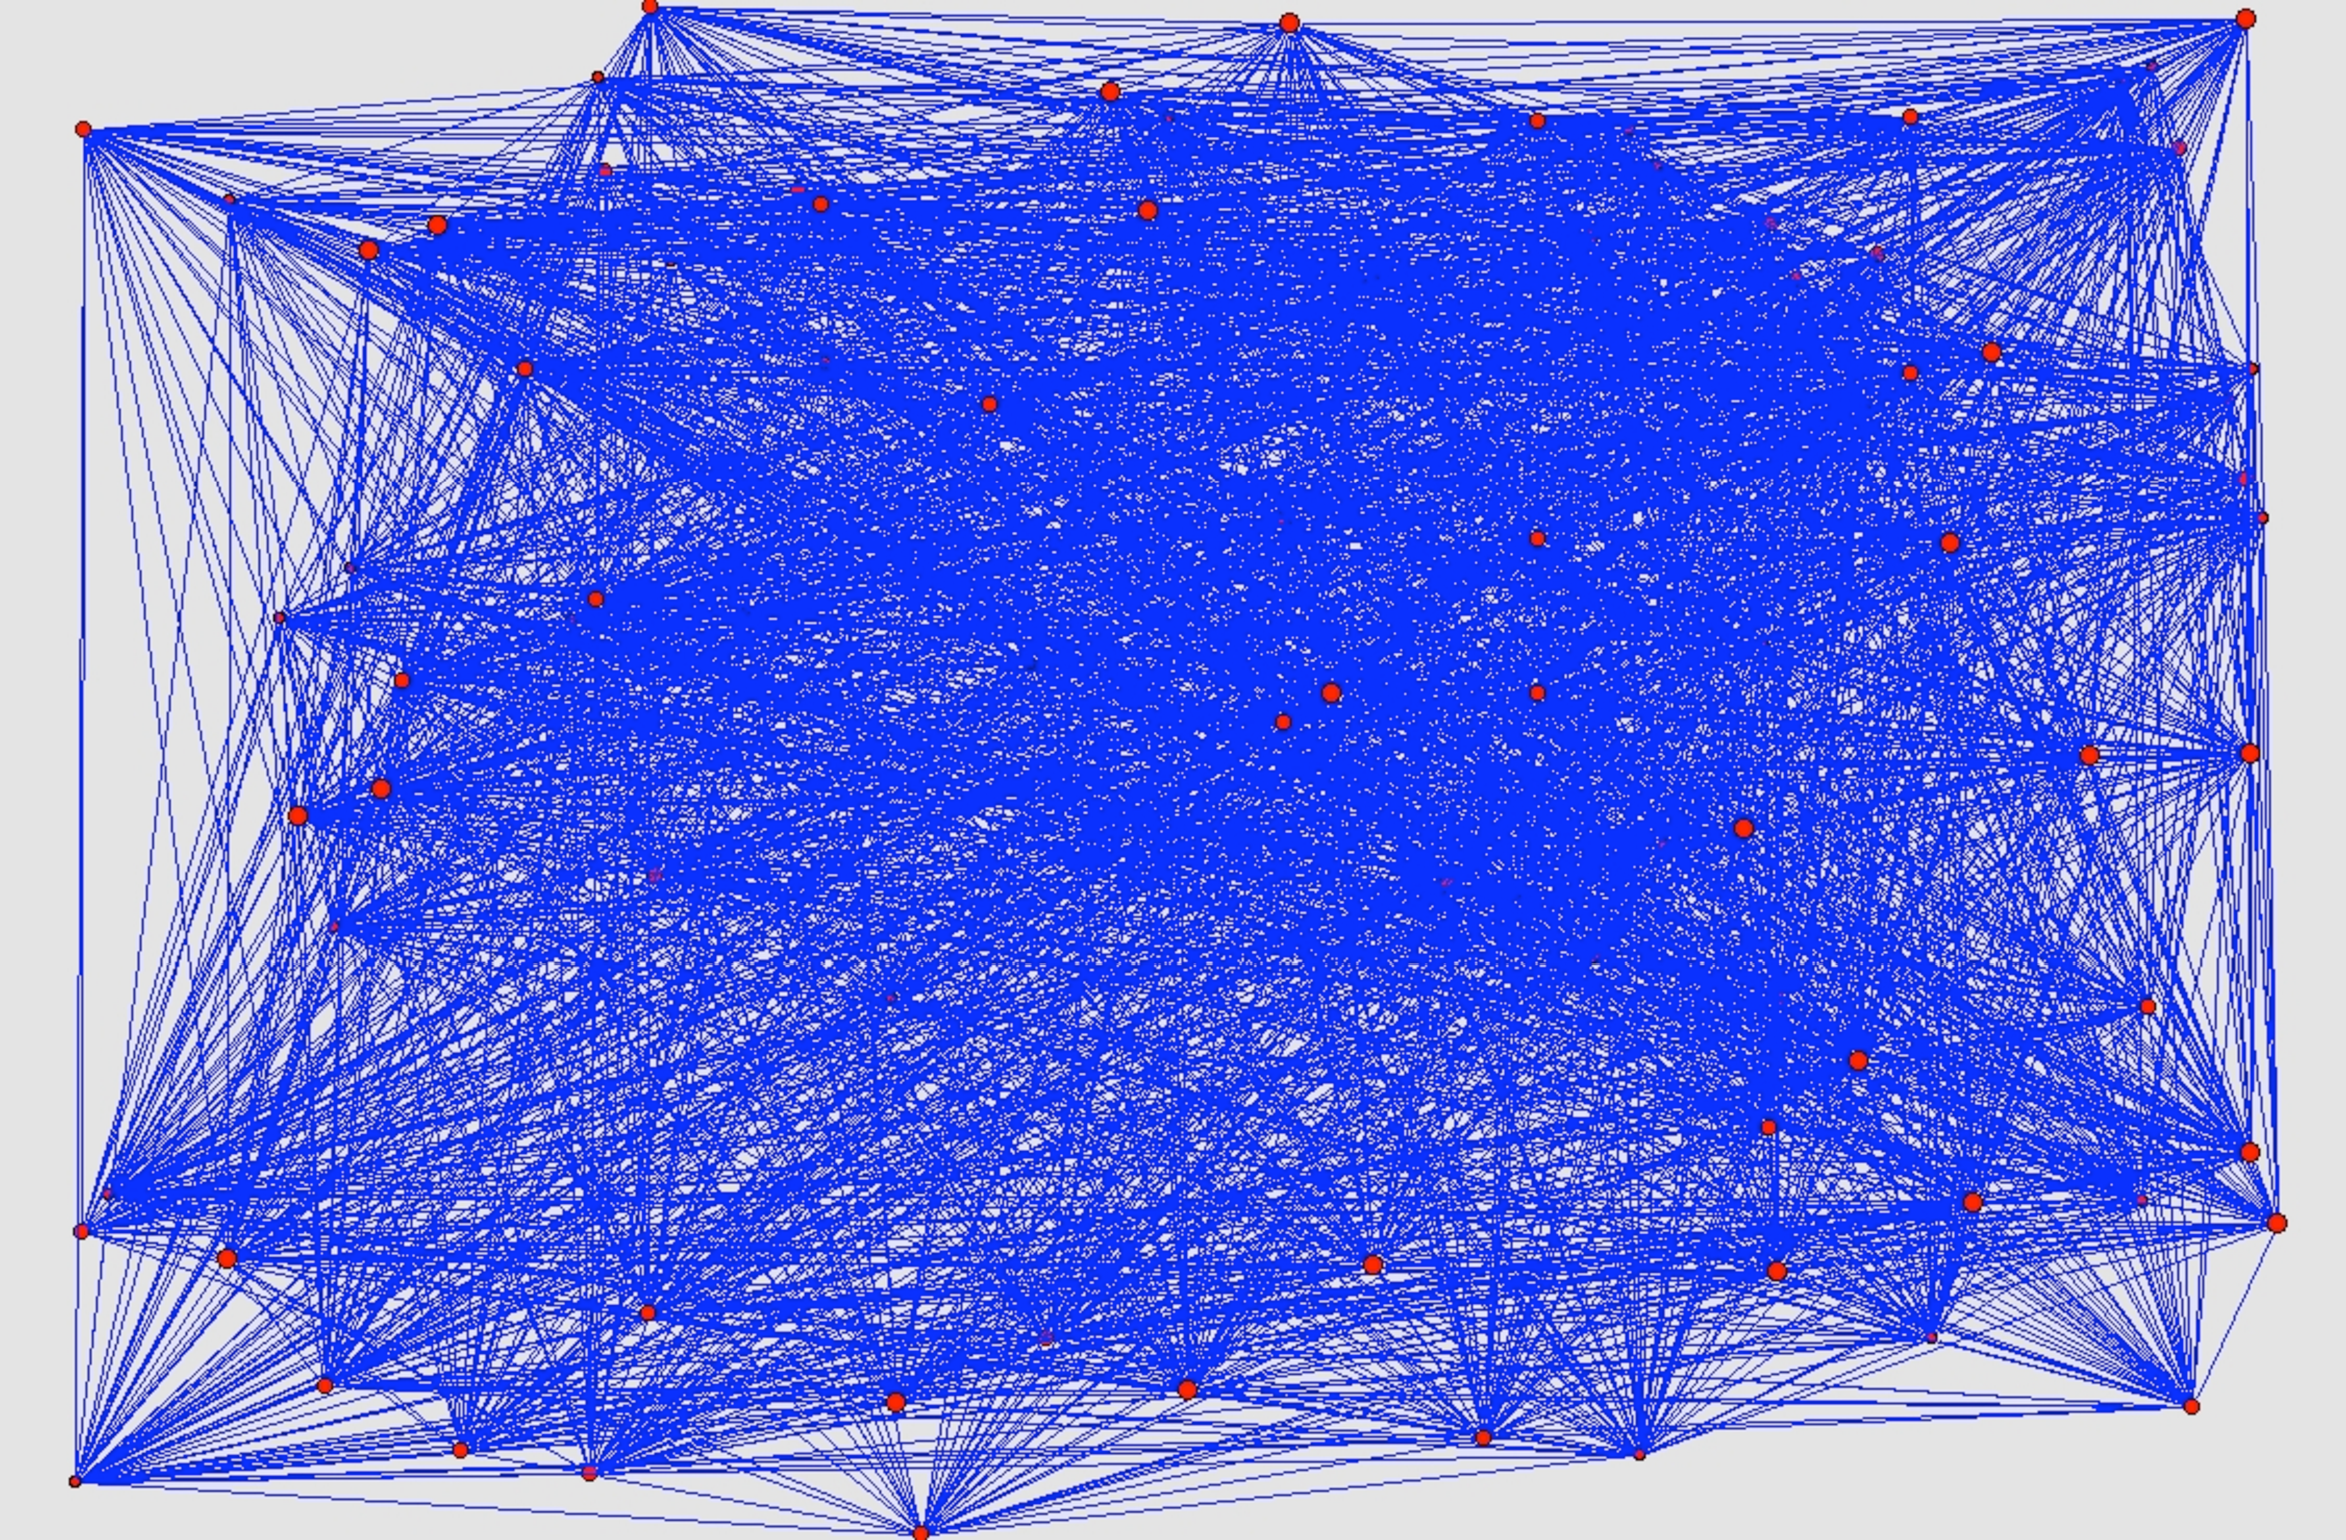
\includegraphics [scale=0.3]  {figures/Pajek9090.pdf}}
\caption{Graphic representation of the functional connectivity
among regions based on the temporal correlation matrix of the twenty-three
healthy controls, using Pajek software \cite{batagelj_pajek_2004}}
\label{Fig:Pajek}
\end{center}
\end{figure}
\bibliographystyle{ieeetr}
%\bibliography{~/Eclipse/workspace/BiblioTex/bibliojgr}
%\cite{florescu_probability_2014}

\bibliography{bibliojgr}

\end{document}


%%%%%% BIBLIO
